\def\vector#1{\mbox{\boldmath $#1$}}
\section{実験原理}
\subsection{概要}
\begin{figure}[h]
\begin{center}
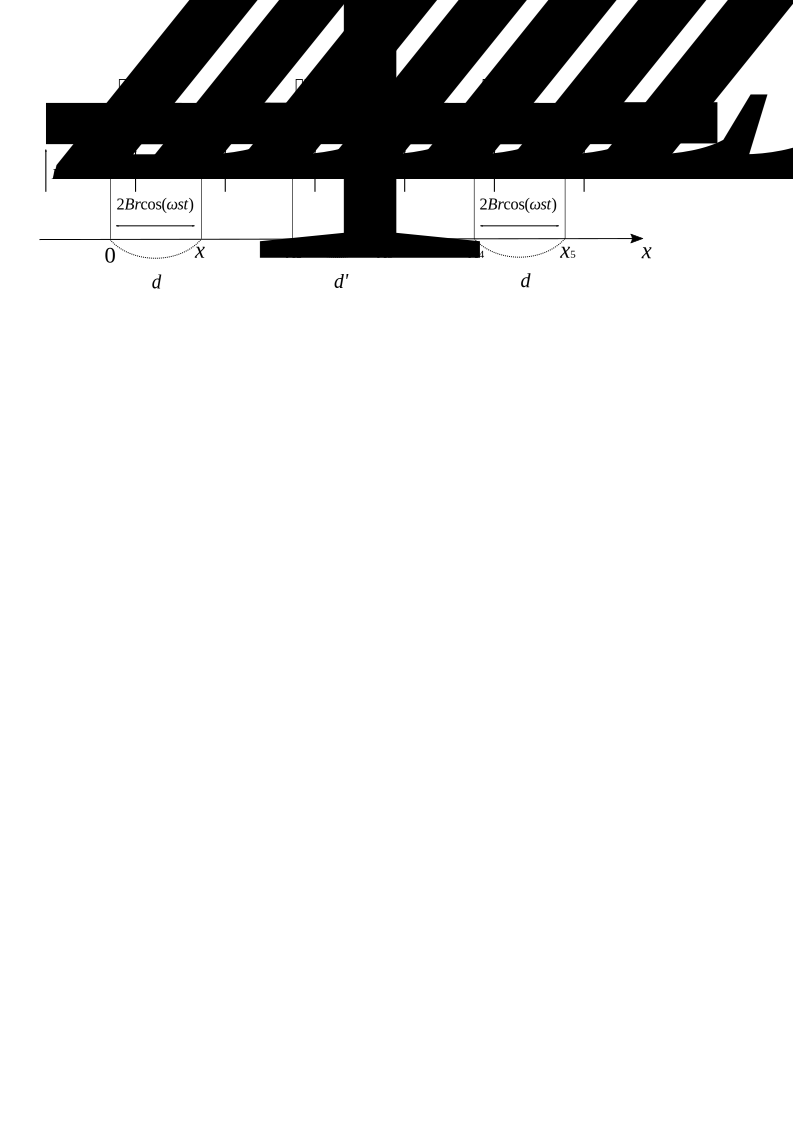
\includegraphics[width=13cm]{pi2flipper/zenntaizu.pdf}
\caption{実験装置の概要}
\end{center}
\end{figure}
今回の実験装置の概要を図に示す。ビームは領域Ⅰから入射し、各領域を通過して、領域Ⅶにある検出器で検出される。領域Ⅰから領域Ⅶにかけて、全体に$z方向の一様磁場B_{z}$がかかっている。領域Ⅱと領域Ⅵには$\pi/2フリッパー$があり、$x方向の振動磁場2B_{r}\cos(\omega_{s}t)$がかかっている。領域Ⅳには位相シフタコイルがあり、$z方向に磁場B+B_{z}$がかかっている。
ここでは、領域Ⅰから、
\begin{align}
{\psi}_{Ⅰ}(x,t)=
\begin{pmatrix}
e^{-i\omega_{z}x/v} \\
0
\end{pmatrix}
e^{ik_{0}x}e^{-i\omega_{0}t}
\end{align}
のような波動関数で表される粒子が、領域Ⅶでどのような状態になるのかを考え、領域Ⅶで干渉が現れることを見る。磁場によるエネルギーが入射波のエネルギーよりも十分に小さいと仮定する。つまり、
\begin{align}
\omega_{0} \gg |{\mu}B_{r}|
\end{align}
と仮定する。このとき、各領域の境界における反射波は無視できる。
\subsection{詳細な計算}
領域Ⅱにおける磁場は
\begin{align}
\bm{B}=2B_{r}\cos(\omega_{s}t)\bm{\hat{x}}+B_{z}\bm{\hat{z}}
\end{align}
であるが、$B_{z} \gg B_{r}$の時は、のちに述べる理由により、$2B_{r}\cos(\omega_{s}t)\bm{\hat{x}} \to  B_{r}\cos(\omega_{s}t)\bm{\hat{x}}+B_{r}\sin(\omega_{s}t)\bm{\hat{y}}$とできる。ゆえに、領域Ⅱにおける磁場は
\begin{align}
\bm{B}=B_{r}\cos(\omega_{s}t)\bm{\hat{x}}+B_{r}\sin(\omega_{s}t)\bm{\hat{y}}+B_{z}\bm{\hat{z}}
\end{align}
であるとする。
\begin{align}
\omega_{r}=|{\mu}B_{r}|
\end{align}
\begin{align}
\omega_{z}=|{\mu}B_{z}|
\end{align}
とする。この時、領域Ⅱにおけるシュレディンガー方程式は
\begin{align}
i\frac{\partial {\psi}_{Ⅱ}(x,t)}{\partial t}=\left(-\frac{1}{2m}\frac{\partial^2}{\partial x^2}+\omega_{r}\cos(\omega_{s}t){\sigma}_{x}+\omega_{r}\sin(\omega_{s}t){\sigma}_{y}+{\hbar}\omega_{z}{\sigma}_{z}\right){\psi}_{Ⅱ}(x,t)
\end{align}
と書ける。ここで、
\begin{align}
\omega_{r}\cos(\omega_{s}t){\sigma}_{x}+\omega_{r}\sin(\omega_{s}t){\sigma}_{y}+\omega_{z}{\sigma}_{z}=
\begin{pmatrix}
\omega_{z} &\omega_{r}e^{-i\omega_{s}t} \\
\omega_{r}e^{i\omega_{s}t} &-\omega_{z}
\end{pmatrix}
\end{align}
$と書ける。角速度\omega_{s}でz軸の周りに回転するユニタリー変換$
\begin{align}
U_{T}=\exp(i\omega_{s}t{\sigma}_{z}/2)=
\begin{pmatrix}
e^{i\omega_{s}t/2} &0 \\
0 &e^{-i\omega_{s}t/2}
\end{pmatrix}
\end{align}
をもちいて
\begin{align}
U_{T}\begin{pmatrix}
\omega_{z} &\omega_{r}e^{-i\omega_{s}t} \\
\omega_{r}e^{i\omega_{s}t} &-\omega_{z}
\end{pmatrix}U_{T}^{\dagger}=
\begin{pmatrix}
\omega_{z} &\omega_{r} \\
\omega_{r} &-\omega_{z}
\end{pmatrix}
\end{align}
が成り立つ。
\begin{align}
{\psi}_{R}(x,t)=U_{T}{\psi}(x,t)
\end{align}
$とすると{\psi}_{R}(x,t)の満たすシュレディンガー方程式は$
\begin{align}
i\frac{\partial {\psi}_{R}(x,t)}{\partial t}=\left(-\frac{1}{2m}\frac{\partial^2}{\partial x^2}+\omega_{r}{\sigma}_{x}+\left(\omega_{z}-\frac{1}{2}\omega_{s}\right){\sigma}_{z}\right){\psi}_{R}(x,t)
\end{align}
となる。いま、共鳴条件
\begin{align}
{\epsilon}=\frac{1}{2}\omega_{s}-\omega_{z}=0
\end{align}
が成り立っているとする。この時、シュレディンガー方程式は
\begin{align}
i\frac{\partial {\psi}_{R}(x,t)}{\partial t}=\left(-\frac{1}{2m}\frac{\partial^2}{\partial x^2}+\omega_{r}{\sigma}_{x}\right){\psi}_{R}(x,t)
\end{align}
いま、
\begin{align}
U_{D}=\exp(i{\pi}{\sigma}_{y}/4)=
\begin{pmatrix}
1/\sqrt{2} &1/\sqrt{2} \\
-1/\sqrt{2} &1/\sqrt{2}
\end{pmatrix}
\end{align}
というユニタリー変換を用いると、
\begin{align}
U_{D}{\sigma}_{x}U_{D}^{\dagger}={\sigma}_{z}
\end{align}
が成り立つ。
\begin{align}
{\psi}_{D}(x,t)=U_{D}{\psi}_{R}(x,t)
\end{align}
$とすると、{\psi}_{D}(x,t)の満たすシュレーディンガー方程式は$
\begin{align}
i\frac{\partial {\psi}_{D}(x,t)}{\partial t}=\left(-\frac{1}{2m}\frac{\partial^2}{\partial x^2}+\omega_{r}{\sigma}_{z}\right){\psi}_{D}(x,t)
\end{align}
$この方程式の解のうち、エネルギー固有値がE_{n}=\omega_{n}であるものは$
\begin{align}
{\psi}_{D}(x,t) =
\begin{pmatrix}
A_{n}^{+}e^{ik_{n}^{+}x}+B_{n}^{+}e^{-ik_{n}^{+}x}  \\
A_{n}^{-}e^{ik_{n}^{-}x}+B_{n}^{-}e^{-ik_{n}^{-}x}
\end{pmatrix}
e^{-i\omega_{n}t}
\end{align}
ここで、
\begin{align}
\frac{{k_{n}^{\pm}}^2}{2m}{\pm}\omega_{r}=E_{n}
\end{align}
が成り立つ。ゆえに、領域Ⅱにおける波動関数は
\begin{align}
{\psi}_{Ⅱ}(x,t)=U_{T}^{\dagger}U_{D}^{\dagger}{\psi}_{D}(x,t)=\frac{1}{\sqrt{2}}
\begin{pmatrix}
\left[(A_{n}^{+}e^{ik_{n}^{+}x}+B_{n}^{+}e^{-ik_{n}^{+}x})+(A_{n}^{-}e^{ik_{n}^{-}x}+B_{n}^{-}e^{-ik_{n}^{-}x})\right]e^{-i(\omega_{n}+\omega_{s}/2)t} \\
\left[(A_{n}^{+}e^{ik_{n}^{+}x}+B_{n}^{+}e^{-ik_{n}^{+}x})-(A_{n}^{-}e^{ik_{n}^{-}x}+B_{n}^{-}e^{-ik_{n}^{-}x})\right]e^{-i(\omega_{n}-\omega_{s}/2)t}
\end{pmatrix}
\end{align}

いま、入射波、すなわち領域Ⅰにおける波動関数を
\begin{align}
{\psi}_{Ⅰ}(x,t)=
\begin{pmatrix}
e^{-i\omega_{z}x/v} \\
0
\end{pmatrix}
e^{ik_{0}x}e^{-i\omega_{0}t}
\end{align}
$とする。ここで、v={k_{0}}/{m}であり、$
\begin{align}
\frac{k_{0}^2}{2m}=E_{0}=\omega_{0}
\end{align}
$が成り立つ。x=0における接続条件により、以下の4つの式が任意のtについて成り立つ。$
\begin{align}
e^{-i\omega_{0}t}=\left[(A_{n}^{+}+B_{n}^{+})+(A_{n}^{-}+B_{n}^{-})\right]e^{-i(\omega_{n}+\omega_{s}/2)t}
\end{align}
\begin{align}
0=\left[(A_{n}^{+}+B_{n}^{+})-(A_{n}^{-}+B_{n}^{-})\right]e^{-i(\omega_{n}-\omega_{s}/2)t}
\end{align}
\begin{align}
(k_{0}-\omega_{z}/v)e^{-i\omega_{0}t}=\left[k_{n}^{+}(A_{n}^{+}-B_{n}^{+})+k_{n}^{-}(A_{n}^{-}-B_{n}^{-})\right]e^{-i(\omega_{n}+\omega_{s}/2)t}
\end{align}
\begin{align}
0=\left[k_{n}^{+}(A_{n}^{+}-B_{n}^{+})-k_{n}^{-}(A_{n}^{-}-B_{n}^{-})\right]e^{-i(\omega_{n}-\omega_{s}/2)t}
\end{align}
これにより、
\begin{align}
\omega_{n}=\omega_{0}-\omega_{s}/2
\end{align}
$を満たすn以外のnについて$
\begin{align}
A_{n}^{+}=B_{n}^{+}=A_{n}^{-}=B_{n}^{-}=0
\end{align}
となる。また、
\begin{align}
\omega_{n}=\omega_{0}-\omega_{s}/2
\end{align}
$を満たすnを1とすると、A_{1}^{\pm},B_{1}^{\pm}は0ではない。以上から、$
\begin{align}
{\psi}_{Ⅱ}(x,t) 
=&\frac{1}{\sqrt{2}}
\begin{pmatrix}
\left[(A_{1}^{+}e^{ik_{1}^{+}x}+B_{1}^{+}e^{-ik_{1}^{+}x})+(A_{1}^{-}e^{ik_{1}^{-}x}+B_{1}^{-}e^{-ik_{1}^{-}x})\right]e^{-i(\omega_{1}+\omega_{s}/2)t} \\
\left[(A_{1}^{+}e^{ik_{1}^{+}x}+B_{1}^{+}e^{-ik_{1}^{+}x})-(A_{1}^{-}e^{ik_{1}^{-}x}+B_{1}^{-}e^{-ik_{1}^{-}x})\right]e^{-i(\omega_{1}-\omega_{s}/2)t}
\end{pmatrix}
\end{align}
$ここで、A_{1}^{+}/\sqrt{2}などを、A_{1}^{+}などと取り直して$
\begin{align}
{\psi}_{Ⅱ}(x,t) 
=&\begin{pmatrix}
\left[(A_{1}^{+}e^{ik_{1}^{+}x}+B_{1}^{+}e^{-ik_{1}^{+}x})+(A_{1}^{-}e^{ik_{1}^{-}x}+B_{1}^{-}e^{-ik_{1}^{-}x})\right]e^{-i\omega_{0}t} \\
\left[(A_{1}^{+}e^{ik_{1}^{+}x}+B_{1}^{+}e^{-ik_{1}^{+}x})-(A_{1}^{-}e^{ik_{1}^{-}x}+B_{1}^{-}e^{-ik_{1}^{-}x})\right]e^{-i(\omega_{0}-\omega_{s})t}
\end{pmatrix}
\end{align}
$透過波、すなわち領域Ⅲにおける波動関数のうち、エネルギー固有値がE_{n}であるものは以下のようなものである。$
\begin{align}
{\psi}_{Ⅲ}(x,t)=
\begin{pmatrix}
C_{n}^{+}e^{iK_{n}^{+}x} \\
C_{n}^{-}e^{iK_{n}^{-}x}
\end{pmatrix}
e^{-i\omega_{n}t}
\end{align}
ここで
\begin{align}
\frac{{K_{n}^{\pm}}^2}{2m}{\pm}\omega_{z}=\omega_{n}
\end{align}
$が成り立つ。x=dにおける接続より、以下の4つの式が任意のtについて成り立つ。$
\begin{align}
C_{n}^{+}e^{iK_{n}^{+}d}e^{-i\omega_{n}t}=\left[(A_{1}^{+}e^{ik_{1}^{+}d}+B_{1}^{+}e^{-ik_{1}^{+}d})+(A_{1}^{-}e^{ik_{1}^{-}d}+B_{1}^{-}e^{-ik_{1}^{-}d})\right]e^{-i\omega_{0}t}
\end{align}
\begin{align}
C_{n}^{-}e^{iK_{n}^{-}d}e^{-i\omega_{n}t}=\left[(A_{1}^{+}e^{ik_{1}^{+}d}+B_{1}^{+}e^{-ik_{1}^{+}d})-(A_{1}^{-}e^{ik_{1}^{-}d}+B_{1}^{-}e^{-ik_{1}^{-}d})\right]e^{-i(\omega_{0}-\omega_{s})t}
\end{align}
\begin{align}
iK_{n}^{+}C_{n}^{+}e^{iK_{n}^{+}d}e^{-i\omega_{n}t}=\left[ik_{1}^{+}(A_{1}^{+}e^{ik_{1}^{+}d}-B_{1}^{+}e^{-ik_{1}^{+}d})+ik_{1}^{-}(A_{1}^{-}e^{ik_{1}^{-}d}-B_{1}^{-}e^{-ik_{1}^{-}d})\right]e^{-i\omega_{0}t}
\end{align}
\begin{align}
iK_{n}^{-}C_{n}^{-}e^{iK_{n}^{-}d}e^{-i\omega_{n}t}=\left[ik_{1}^{+}(A_{1}^{+}e^{ik_{1}^{+}d}-B_{1}^{+}e^{-ik_{1}^{+}d})-ik_{1}^{-}(A_{1}^{-}e^{ik_{1}^{-}d}-B_{1}^{-}e^{-ik_{1}^{-}d})\right]e^{-i(\omega_{0}-\omega_{s})t}
\end{align}
$いま、\omega_{n}=\omega_{0}でも\omega_{n}=\omega_{0}-\omega_{s}でもないnについては$
\begin{align}
C_{n}^{+}=C_{n}^{-}=0
\end{align}
が成り立つ。ゆえに、
\begin{align}
\omega_{2}=\omega_{0}-\omega_{s}
\end{align}
$とすると、残るのはnが0と2だけで、さらに$
\begin{align}
C_{0}^{-}=C_{2}^{+}=0
\end{align}
透過波はこれらを重ね合わせた
\begin{align}
{\psi}_{Ⅲ}(x,t)=
\begin{pmatrix}
C_{0}^{+}e^{iK_{0}^{+}x} \\
0
\end{pmatrix}
e^{-i\omega_{0}t}+
\begin{pmatrix}
0 \\
C_{2}^{-}e^{iK_{2}^{-}x}
\end{pmatrix}
e^{-i\omega_{2}t}
=\begin{pmatrix}
C_{0}^{+}e^{iK_{0}^{+}x}e^{-i\omega_{0}t} \\
C_{2}^{-}e^{iK_{2}^{-}x}e^{-i(\omega_{0}-\omega_{s})t}
\end{pmatrix}
\end{align}
である。ここで、
\begin{align}
\frac{{K_{n}^{\pm}}^2}{2m}{\pm}\omega_{z}=\omega_{n}
\end{align}
により、
\begin{align}
\frac{{K_{0}^{+}}^2}{2m}+\omega_{z}=\omega_{0}
\end{align}
\begin{align}
\frac{{K_{2}^{-}}^2}{2m}-\omega_{z}=\omega_{0}-\omega_{s}
\end{align}
よって
\begin{align}
K_{0}^{+}=\sqrt{2m(\omega_{0}-\omega_{z})}{\simeq}k_{0}-\omega_{z}/v
\end{align}
\begin{align}
K_{2}^{-}=\sqrt{2m((\omega_{0}-\omega_{s})+\omega_{z})}{\simeq}k_{0}+(\omega_{z}-\omega_{s})/v
\end{align}
よって
\begin{align}
{\psi}_{Ⅲ}(x,t)=
\begin{pmatrix}
C_{0}^{+}e^{iK_{0}^{+}x}e^{-i\omega_{0}t} \\
C_{2}^{-}e^{iK_{2}^{-}x}e^{-i(\omega_{0}-\omega_{s})t}
\end{pmatrix}
{\simeq}
\begin{pmatrix}
C_{0}^{+}e^{i(k_{0}-\omega_{z}/v)x}e^{-i\omega_{0}t} \\
C_{2}^{-}e^{i(k_{0}+(\omega_{z}-\omega_{s})/v)x}e^{-i(\omega_{0}-\omega_{s})t}
\end{pmatrix}=
\begin{pmatrix}
C_{0}^{+}e^{i(-\omega_{z}/v)x} \\
C_{2}^{-}e^{i((\omega_{z}-\omega_{s})/v)x}e^{i\omega_{s}t}
\end{pmatrix}
e^{ik_{0}x}e^{-i\omega_{0}t}
\end{align}
ここで、共鳴条件
\begin{align}
\omega_{s}=2\omega_{z}
\end{align}
により、
\begin{align}
{\psi}_{Ⅲ}(x,t)=& \notag
\begin{pmatrix}
C_{0}^{+}e^{i(-\omega_{z}/v)x} \\
C_{2}^{-}e^{i(-\omega_{z}/v)x}e^{i\omega_{s}t}
\end{pmatrix}
e^{ik_{0}x}e^{-i\omega_{0}t}\\ \notag
=&\begin{pmatrix}
C_{0}^{+} \\
C_{2}^{-}e^{i\omega_{s}t}
\end{pmatrix}
e^{-i\omega_{z}/vx}e^{ik_{0}x}e^{-i\omega_{0}t}\\ 
=&\begin{pmatrix}
\cos(\omega_{r}d/v) \\
-i\sin(\omega_{r}d/v)e^{i\omega_{s}t}
\end{pmatrix}
e^{-i\omega_{z}/vx}e^{ik_{0}x}e^{-i\omega_{0}t}  
=&\begin{pmatrix}
\cos(\omega_{r}d/v)e^{i(k_{0}-\omega_{z}/v)x}e^{-i\omega_{0}t} \\
-i\sin(\omega_{r}d/v)e^{i(k_{0}-\omega_{z}/v)x}e^{-i(\omega_{0}-\omega_{s})t} 
\end{pmatrix}
\end{align}

$領域ⅢとⅣの境界x=l_{1}における波動関数は$
\begin{align}
{\psi}_{Ⅲ}(x=l_{1},t)=
\begin{pmatrix}
\cos(\omega_{r}d/v)e^{i(k_{0}-\omega_{z}/v)l_{1}}e^{-i\omega_{0}t} \\
-i\sin(\omega_{r}d/v)e^{i(k_{0}-\omega_{z}/v)l_{1}}e^{-i(\omega_{0}-\omega_{s})t}
\end{pmatrix}
\end{align}
$領域Ⅳにおける磁場をB=(\omega+\omega_{z})/{\mu}とすると、この領域ではスピン上成分が波数$
\begin{align}
k_{0}-(\omega+\omega_{z})/v
\end{align}
スピン下成分が波数
\begin{align}
k_{0}+((\omega+\omega_{z})-\omega_{s})/v=k_{0}+(\omega-\omega_{z})/v
\end{align}
で進んでいくので、領域Ⅳにおける波動関数は、
\begin{align}
{\psi}_{Ⅳ}(x,t)=
\begin{pmatrix}
\cos(\omega_{r}d/v)e^{i(k_{0}-\omega_{z}/v)l_{1}}e^{i(k_{0}-(\omega+\omega_{z})/v)(x-l_{1})}e^{-i\omega_{0}t} \\
-i\sin(\omega_{r}d/v)e^{i(k_{0}-\omega_{z}/v)l_{1}}e^{i(k_{0}+(\omega-\omega_{z})/v)(x-l_{1})}e^{-i(\omega_{0}-2\omega_{z})t}
\end{pmatrix}
\end{align}

領域Ⅴでは、両成分とも波数
\begin{align}
k_{0}-\omega_{z}/v
\end{align}
で進んでいくので、領域Ⅴにおける波動関数は
\begin{align}
{\psi}_{Ⅴ}(x,t)=
\begin{pmatrix}
\cos(\omega_{r}d/v)e^{i(k_{0}-\omega_{z}/v)l_{1}}e^{i(k_{0}-(\omega+\omega_{z})/v)(l_{2}-l_{1})}e^{i(k_{0}-\omega_{z}/v)(x-l_{2})}e^{-i\omega_{0}t} \\
-i\sin(\omega_{r}d/v)e^{i(k_{0}-\omega_{z}/v)l_{1}}e^{i(k_{0}+(\omega-\omega_{z})/v)(l_{2}-l_{1})}e^{i(k_{0}-\omega_{z}/v)(x-l_{2})}e^{-i(\omega_{0}-2\omega_{z})t}
\end{pmatrix}
\end{align}

$領域ⅤとⅥの境界x=l_{3}における波動関数は$
\begin{align}
{\psi}_{Ⅴ}(x=l_{3},t)=
\begin{pmatrix}
{\alpha}e^{-i\omega_{0}t} \\
{\beta}e^{-i(\omega_{0}-2\omega_{z})t}
\end{pmatrix}
\end{align}
ここで、
\begin{align}
{\alpha}=\cos\left(\omega_{r}d/v\right)e^{i(k_{0}-\omega_{z}/v)l_{1}}e^{i\left(k_{0}-(\omega+\omega_{z})/v\right)(l_{2}-l_{1})}e^{i\left(k_{0}-\omega_{z}/v\right)(l_{3}-l_{2})}
\end{align}
\begin{align}
{\beta}=-i\sin\left(\omega_{r}d/v\right)e^{i(k_{0}-\omega_{z}/v)l_{1}}e^{i\left(k_{0}+(\omega-\omega_{z})/v\right)(l_{2}-l_{1})}e^{i\left(k_{0}-\omega_{z}/v\right)(l_{3}-l_{2})}
\end{align}
$領域Ⅵにおける波動関数のうち、エネルギーがE_{n}であるものは$
\begin{align}
{\psi}_{Ⅵ}(x,t)=
\begin{pmatrix}
(D_{n}^{+}e^{ik_{n}^{+}x}+D_{n}^{-}e^{ik_{n}^{-}x} )e^{-i(\omega_{n}+\omega_{z})t}\\
(D_{n}^{+}e^{ik_{n}^{+}x}-D_{n}^{-}e^{ik_{n}^{-}x} )e^{-i(\omega_{n}-\omega_{z})t}
\end{pmatrix}
\end{align}
である。ここで、
\begin{align}
\frac{{k_{n}^{\pm}}^2}{2m}{\pm}\omega_{r}=\omega_{n}
\end{align}
$が成り立つ。x=l_{3}における接続により$
\begin{align}
{\alpha}e^{-i\omega_{0}t}=\left(D_{n}^{+}e^{ik_{n}^{+}l_{3}}+D_{n}^{-}e^{ik_{n}^{-}l_{3}}\right)e^{-i\left(\omega_{n}+\omega_{z}\right)t}
\end{align}
\begin{align}
{\beta}e^{-i(\omega_{0}-2\omega_{z})t}=\left(D_{n}^{+}e^{ik_{n}^{+}l_{3}}-D_{n}^{-}e^{ik_{n}^{-}l_{3}}\right)e^{-i\left(\omega_{n}-\omega_{z}\right)t}
\end{align}
すると
\begin{align}
\omega_{2}=\omega_{0}-\omega_{z}
\end{align}
$として、n=2のもの以外は0になる。$
\begin{align}
{\alpha}=\left(D_{2}^{+}e^{ik_{2}^{+}l_{3}}+D_{2}^{-}e^{ik_{2}^{-}l_{3}}\right)
\end{align}
\begin{align}
{\beta}=\left(D_{2}^{+}e^{ik_{2}^{+}l_{3}}-D_{2}^{-}e^{ik_{2}^{-}l_{3}}\right)
\end{align}
よって
\begin{align}
D_{2}^{+}=\frac{1}{2}e^{-ik_{2}^{+}l_{3}}({\alpha}+{\beta})
\end{align}
\begin{align}
D_{2}^{-}=\frac{1}{2}e^{-ik_{2}^{-}l_{3}}({\alpha}-{\beta})
\end{align}
ゆえに、領域Ⅵにおける波動関数は
\begin{align}
{\psi}_{Ⅵ}(x,t)=\frac{1}{2}
\begin{pmatrix}
\left(({\alpha}+{\beta})e^{ik_{2}^{+}(x-l_{3})}+({\alpha}-{\beta})e^{ik_{2}^{-}(x-l_{3})}\right)e^{-i\omega_{0}t}\\
\left(({\alpha}+{\beta})e^{ik_{2}^{+}(x-l_{3})}-({\alpha}-{\beta})e^{ik_{2}^{-}(x-l_{3})}\right)e^{-i(\omega_{0}-2\omega_{z})t}
\end{pmatrix}
\end{align}

領域Ⅶでは両成分とも波数
\begin{align}
k_{0}-\omega_{z}/v
\end{align}
で進んでいくので、波動関数は
\begin{align}
{\psi}_{Ⅶ}(x,t)=\frac{1}{2}
\begin{pmatrix}
\left(({\alpha}+{\beta})e^{ik_{2}^{+}(l_{4}-l_{3})}+({\alpha}-{\beta})e^{ik_{2}^{-}(l_{4}-l_{3})}\right)e^{i(k_{0}-\omega_{z}/v)(x-l_{4})}e^{-i\omega_{0}t}\\
\left(({\alpha}+{\beta})e^{ik_{2}^{+}(l_{4}-l_{3})}-({\alpha}-{\beta})e^{ik_{2}^{-}(l_{4}-l_{3})}\right)e^{i(k_{0}-\omega_{z}/v)(x-l_{4})}e^{-i(\omega_{0}-2\omega_{z})t}
\end{pmatrix}
\end{align}
スピン上成分の絶対値の2乗は
\begin{align}
\left|({\psi}_{Ⅶ}(x,t))_{+}\right|^2=\frac{1}{4}\left|({\alpha}+{\beta})e^{ik_{2}^{+}(l_{4}-l_{3})}+({\alpha}-{\beta})e^{ik_{2}^{-}(l_{4}-l_{3})}\right|^2
\end{align}
ここで、
\begin{align}
\frac{{k_{n}^{\pm}}^2}{2m}{\pm}\omega_{r}=\omega_{n}
\end{align}
により、
\begin{align}
\frac{{k_{2}^{\pm}}^2}{2m}{\pm}\omega_{r}=\omega_{2}=\omega_{0}-\omega_{z}
\end{align}
\begin{align}
k_{2}^{\pm}{\simeq}k_{0}-\frac{\omega_{z}{\pm}\omega_{r}}{v}
\end{align}
よって
\begin{align}
|({\psi}_{Ⅶ}(x,t))_{+}|^2 
&=\frac{1}{4}\left|({\alpha}+{\beta})e^{-i\omega_{r}/v(l_{4}-l_{3})}+({\alpha}-{\beta})e^{i\omega_{r}/v(l_{4}-l_{3})}\right|^2 \notag \\
&=\left|{\alpha}\cos\left(\frac{\omega_{r}}{v}(l_{4}-l_{3})\right)-i{\beta}\sin\left(\frac{\omega_{r}}{v}(l_{4}-l_{3})\right)\right|^2 \notag \\
&=\left|e^{i(k_{0}-(\omega+\omega_{z})/v)(l_{2}-l_{1})}\cos\left(\frac{\omega_{r}}{v}d\right)\cos\left(\frac{\omega_{r}}{v}(l_{4}-l_{3})\right)\right. \\
&\left. \hspace{2cm} -e^{i(k_{0}+(\omega-\omega_{z})/v)(l_{2}-l_{1})}\sin\left(\frac{\omega_{r}}{v}d\right)\sin\left(\frac{\omega_{r}}{v}(l_{4}-l_{3})\right)\right|^2
\end{align}
$ここで、l_{4}-l_{3}=dである。また、l_{2}-l_{1}=d'として、$
\begin{align}
|({\psi}_{Ⅶ}(x,t))_{+}|^2   
&=\left|e^{-i\omega d'/v}\cos^2\left(\frac{\omega_{r}}{v}d\right) -e^{i\omega d'/v}\sin^2\left(\frac{\omega_{r}}{v}d\right)\right|^2 \notag \\
&={\left(\cos\left(\frac{\omega}{v}d'\right)\cos^2\left(\frac{\omega_{r}}{v}d\right)-\cos\left(\frac{\omega}{v}d'\right)\sin^2\left(\frac{\omega_{r}}{v}d\right)\right)}^2 +{\left(\sin\left(\frac{\omega}{v}d'\right)\cos^2\left(\frac{\omega_{r}}{v}d\right)+\sin\left(\frac{\omega}{v}d'\right)\sin^2\left(\frac{\omega_{r}}{v}d\right)\right)}^2\notag \\
&=\cos^4\left(\frac{\omega_{r}}{v}d\right)+\sin^4\left(\frac{\omega_{r}}{v}d\right)  -2\left(\cos\left(\frac{\omega}{v}d'\right)\cos\left(\frac{\omega}{v}d'\right)-\sin\left(\frac{\omega}{v}d'\right)\sin\left(\frac{\omega}{v}d'\right)\right)\cos^2\left(\frac{\omega_{r}}{v}d\right)\sin^2\left(\frac{\omega_{r}}{v}d\right) \notag \\
&=\cos^4\left(\frac{\omega_{r}}{v}d\right)+\sin^4\left(\frac{\omega_{r}}{v}d\right) -2\cos\left(\frac{2\omega}{v}d'\right)\cos^2\left(\frac{\omega_{r}}{v}d\right)\sin^2\left(\frac{\omega_{r}}{v}d\right) \notag \\
&=\left(\cos^2\left(\frac{\omega_{r}}{v}d\right)+\sin^2\left(\frac{\omega_{r}}{v}d\right)\right)^2 -2\left(1+\cos\left(\frac{2\omega}{v}d'\right)\right)\cos^2\left(\frac{\omega_{r}}{v}d\right)\sin^2\left(\frac{\omega_{r}}{v}d\right)  \notag \\
&=1-4\cos^2\left(\frac{\omega}{v}d'\right)\cos^2\left(\frac{\omega_{r}}{v}d\right)\sin^2\left(\frac{\omega_{r}}{v}d\right) \notag \\
&=1-\cos^2\left(\frac{\omega}{v}d'\right)\sin^2\left(\frac{2\omega_{r}}{v}d\right) 
\end{align}
$ゆえに、領域Ⅳにおける磁場Bの大きさを変えながらビームの下流でスピン上成分の粒子の数を測定すると、干渉が観測できる。$




